\myClearDoublePage
\chapter{Implementation}

The previous section focused on the theoretical approach to designing a tracking module for a receiver, and this chapter will explain the specific practical process and the problems encountered during the process. This project mainly implements the tracking module on a GPS receiver, please note that this is only a separate module and does not realise the full receiver functionality. It also has RF front-end and acquisition modules in the front module, and ranging modules as well as navigation modules in the back module. The project in fact has a hypothetical target device, but based on the current conditions, the main use of VHDL for code writing, as well as behavioural simulation to verify the results, will not be on-board operations.

\section{System Architecture}
\subsection{RF Front-end}

The RF front-end is a device that collects any signals you expect. In this project, we will use \textit{NT1065\_FMC2} as our front-end. This device is designed to receive GPS, GLONASS, Galileo, BeiDou, IRNSS, QZSS and L1, L2, L3, L5, E1, E5a, E5b, E6, B1, B2, B3 bands. It has an FMC(\textit{FPGA Mezzanine Card}) interface, which allows it to have a faster transfer rate to the Xilinx board \cite{RN206}. Figure \ref{fig:nt1065} shows the device's appearance. Here is its key specification table.

\begin{table}[!htbp]
\centering
\caption{Key Specification of \textit{NT1065\_FMC2}}\label{tab:nt1065}
\renewcommand\arraystretch{1.5}
\begin{tabular}{cc}
    \toprule
    Content & Specifications \\
    \midrule
    Chip & NT1065 \\
    Number of channels & 4 \\
    \multirow{2}{*}{Reference frequency sources (MHz)} & TCXO 10 \\
     & TCXO 24.84 \\
    Bit width of ADC (bits) & 2 \\
    \bottomrule
\end{tabular}
\end{table}

\begin{figure}[!htbp]
    \centering
    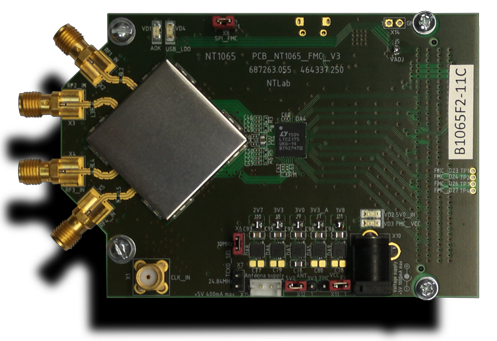
\includegraphics[width=0.8\textwidth]{_IMAGES/fmc-2-nt1065.png}
    \caption{\textit{NT1065\_FMC2}}
    \label{fig:nt1065}
\end{figure}

\subsection{FPGA Board}
The FPGA board is the core module of this project. It will process the acquisition, tracking and navigation stages. The board we choose is \textit{KCU105 Evaluation Board} from \textit{AMD Xilinx}. It's very powerful. Its specification and appearance will be shown below.

\begin{table}[!htbp]
\centering
\caption{Key Specification of \textit{KCU105 Evaluation Board}}
\label{tab:kcu105}
\renewcommand\arraystretch{1.5}
\begin{tabular}{cc}
    \toprule
    Content & Specifications \\
    \midrule
    Chip & XCKU040-2FFVA1156E FPGA \\
    System Logic Cells (K) & 530 \\
    DSP Slices & \num{1920} \\
    Block RAM (Mb) & 21.1 \\
    16.3Gb/s Transceivers & 20 \\
    I/O Pins & 520 \\
    \multirow{3}{*}{Memory} & 2GB DDR4 component memory \\
     & 64MB flash \\
     & 8Kb EEPROM \\
     \bottomrule
\end{tabular}
\end{table}

\begin{figure}[!htbp]
    \centering
    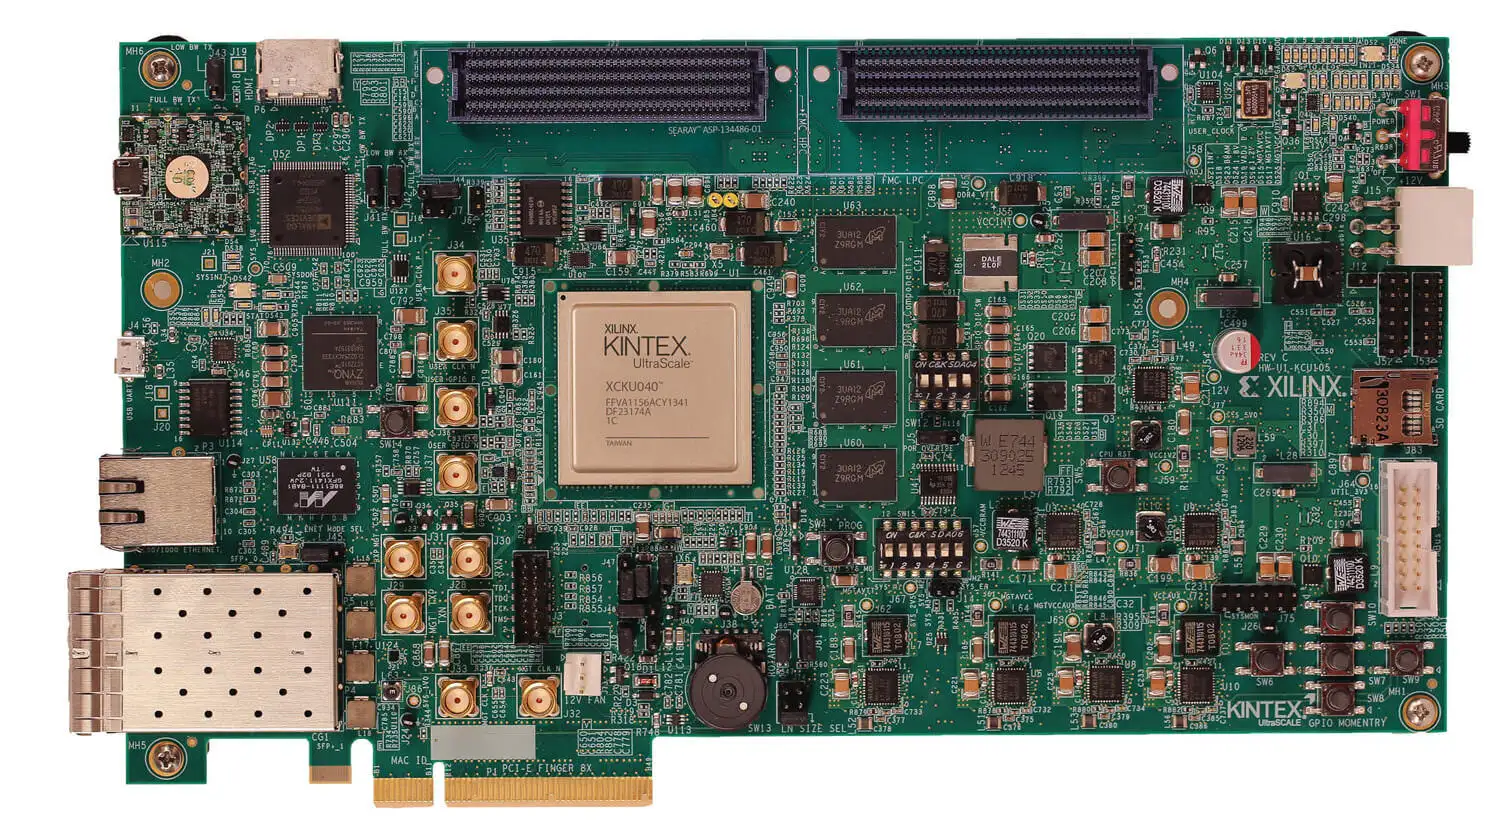
\includegraphics[width=0.8\textwidth]{_IMAGES/KCU105_evaluation_board.png}
    \caption{\textit{KCU105 Evaluation Board}}
    \label{fig:kcu105}
\end{figure}

\section{Develop Environment}
\subsection{Vivado}
As we are planning to use FPGA from \textit{Xilinx}, we are supposed to code in \textit{Vivado}. It is a powerful and versatile integrated development environment (IDE) created by Xilinx for FPGA and SoC development. It offers a comprehensive suite of tools and features for designing, implementing, and programming FPGAs and SoCs, enabling engineers to create custom digital hardware solutions. With its user-friendly interface and advanced design automation capabilities, \textit{Vivado} simplifies the process of hardware design, synthesis, verification, and debugging. It supports a wide range of Xilinx devices, making it a go-to tool for hardware engineers and developers working on cutting-edge applications in industries like telecommunications, aerospace, and embedded systems. The version we use is \textbf{2018.3}. The reason for that is that it is stable but not outdated.

\subsection{ModelSim}
\textit{ModelSim} is used to verify the design. We will run the simulation and check all the waveforms of the key signal. \textit{ModelSim} is a leading digital simulation and verification tool by Mentor Graphics, now a part of Siemens. It's widely used for designing and testing digital systems, enabling engineers to simulate hardware description languages like VHDL and Verilog. \textit{ModelSim} assists in debugging, verification, and validation of complex digital designs in various industries.

\textit{ModelSim} is particularly compatible with Vivado, and when used in conjunction with it, you get twice the result with half the effort, and it can quickly locate code errors.

\subsection{MATLAB}
Matlab is a high-level programming environment and language renowned for its versatility in numerical computing, data analysis, and algorithm development. Used across various fields, from engineering to finance, it offers extensive libraries and tools for modelling, simulation, and solving complex mathematical problems, making it indispensable in research and industry. The reason for using it is to run the \textit{SoftGNSS} to verify my design as well.

\section{Signal Analyse and Pre-process}
At the beginning of the project, the only data known to us were the input signals. Therefore it is very crucial to analyse and pre-process the input signals. I will be using MATLAB to analyse the data and the figure below shows the results of my analysis.

\begin{figure}[!htbp]
    \centering
    \includesvg[width=0.8\textwidth]{_IMAGES/PPT2SVG/signal_info.svg}
    \caption{Signal Analyse}
    \label{fig:sig_info}
\end{figure}

From the frequency domain in figure \ref{fig:sig_info}, we can see the IF is about 14.7025MHz. This is in line with our expectations. Also a perfect spectrum of signals can be seen, proving that I'm picking up the correct GPS signals. We should take note of the histogram, which provides us with a lot of basis. We can calculate the noise floor based on it, and we can also verify that we are reading the right data on the testbench based on its distribution. The following table \ref{tab:dis_sig} shows the distribution information of the input signals.

\begin{table}[!htbp]
\centering
\renewcommand\arraystretch{1.5}
\caption{Distribution Table of the Input Signal}
\label{tab:dis_sig}
\begin{tabular}{ccc}
    \toprule
    Value & Counts & Percentage (\%) \\
    \midrule
    -3 & \num{141278} & 14.22 \\
    -1 & \num{337040} & 33.92 \\
    1 & \num{346219} & 34.84 \\
    3 & \num{169213} & 17.03 \\
    \bottomrule
\end{tabular}
\end{table}

In addition, the basic information will be shown in table \ref{tab:sig_info}.

\begin{table}[!htbp]
\centering
\renewcommand\arraystretch{1.5}
\caption{Basic Infomation of the Signal}
\label{tab:sig_info}
\begin{tabular}{cc}
    \toprule
    \multicolumn{2}{c}{Basic Infomation of the Signal} \\
    \midrule
    IF (MHz) & 14.58 \\
    Sampling frequency (MHz) & 99.375 \\
    Code frequency (MHz) & 1.023 \\
    Data type & int 8 \\
    Samples/code & \num{99375} \\
    Accumulate time (ms) & 1 \\
    \bottomrule
\end{tabular}
\end{table}

\section{Tracking}
Before tracking, we need the acquisition result. The part has been done on the \textit{SoftGNSS}. Here are the results.

\begin{table}[!htbp]
\centering
\renewcommand\arraystretch{1.5}
\caption{Results of the Acquisition}
\label{tab:result_acqu}
\begin{tabular}{cc}
    \toprule
    \multicolumn{2}{c}{Result} \\
    \midrule
    Chopped bits & \num{46500} \\
    PRN (\textnumero) & 2 \\
    IF (MHz) & 14.5778 \\
    Doppler (Hz) & 2200 \\
    Code offset (Chips) & 162 \\
    \bottomrule
\end{tabular}
\end{table}

These results are fed directly into the tracking stage.

\subsection{NCO}
The NCO block is driven by a 99.375MHz signal. Firstly, we need to obtain the FSW. The bit width of the PA is 32 bits and the search frequency is 500Hz. The required carrier frequency is $IF+Doppler$, which is 14.5822MHz. 

However, the code frequency is a bit different. To obtain that, we will first introduce the search frequency. The search frequency allows us to let the local code block slide to determine to inner product. We are expecting to have half a chip more per millisecond, i.e., 0.5 chips/ms. Therefore, the search frequency is 500Hz.Here is the diagram of search frequency.

\begin{figure}[!htbp]
    \centering
    \includesvg[width=0.8\textwidth]{_IMAGES/PPT2SVG/search_frequency.svg}
    \caption{Diagram of Search Frequency}
    \label{fig:search_frequency}
\end{figure}

The required code frequency is $Code\  frequency-Search\ frequency = 1.0225Mhz$ then. Using the equation \ref{equ:nco}, we can determine the proper increment value or FSW.

\begin{equation}
    (increment\ value) = \frac{Requied\ frequency}{Sampling\ frequency} \times 2^{PA\ bit\ width}
\end{equation}

In order to be able to track 10.23MHz C/A codes in the future, the 10.23MHz signal will first be generated using the NCO and a $1/10$ divider will be used to obtain a 1.023MHz signal. Therefore, the FSWs for carrier and code are \num{630239720} and \num{441922422}.

As for the design of VHDL, essentially, the PA is a counter, except that each clock does not increment by 1 but by a specified value based on FSW. It is also possible to set the overflow value. After the overflow value is reached, the counter will be set to 0.

Since we only need two-bit width carrier signals, the lookup table for the NCO will be very simple, as shown in the table below.

\begin{table}[!htbp]
\centering
\renewcommand\arraystretch{1.5}
\caption{LUT of NCO for Generating Carrier}
\label{tab:lut_nco}
\begin{tabular}{ccc}
    \toprule
    Phase (First 3 bits) & \multicolumn{2}{c}{Amplitude} \\
    & Cosine & Sine \\
    \midrule
    000 & 2 & -1 \\
    001 & 2 & 1 \\
    010 & 1 & 2 \\
    011 & -1 & 2 \\
    100 & -2 & 1 \\
    101 & -2 & -1 \\
    110 & -1 & -2 \\
    111 & 1 & -2 \\
    \bottomrule
\end{tabular}
\end{table}

\subsubsection{Simulation and Waveform}
In this subsection, the NCO-related code is simulated and all signals generated by the NCO are shown.

The following figure shows the PA waveform when the NCO generates the C/A code clock signal. As mentioned before, a $10.23MHz-\num{5000}Hz$ signal is generated first, and then a 1/10 divider is used to get $1.023-500Hz$. From the figure, it can be seen that after ten overflows, the C/A code is clocked at 1.024MHz, which is within the acceptable range, although there are errors.

\begin{figure}[!htbp]
    \centering
    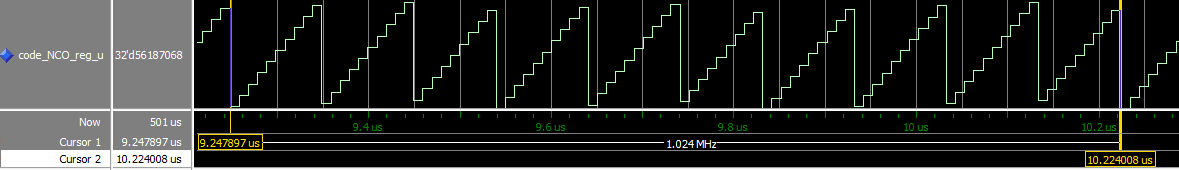
\includegraphics[width=0.8\textwidth]{_IMAGES/nco_code_wave.png}
    \caption{Waveform of NCO for Generating C/A Code}
    \label{fig:nco_code_wave}
\end{figure}

Figure \ref{fig:nco_carrier_wave} shows that using the NCO to generate the carrier signals containing cosine and sine signals which are used to get the I/Q phase of the input signal.

\begin{figure}[!htbp]
    \centering
    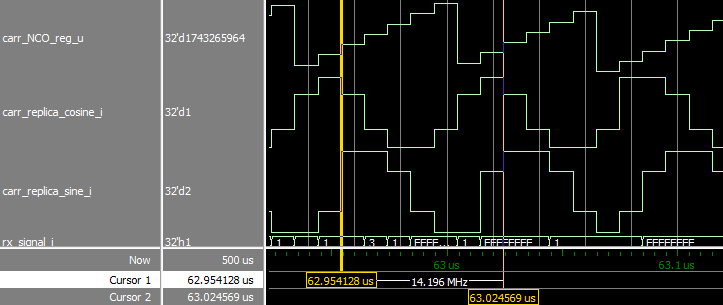
\includegraphics[width=0.8\textwidth]{_IMAGES/nco_carrier_wave.png}
    \caption{Waveform of NCO for Generating Carrier}
    \label{fig:nco_carrier_wave}
\end{figure}

\subsection{Code Generator}
In order to save computational resources on board, I calculated the required PRN code, i.e. PRN \textnumero 2 code, in advance. It is generated through Matlab and stored in VHDL code.

\begin{figure}[!h]
    \centering
    \subfloat[MATLAB]{
        \centering
        \label{fig:prn2_matlab}
        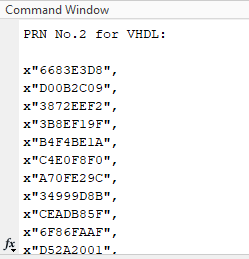
\includegraphics[width=0.3\linewidth]{_IMAGES/prn2_matlab.png}}
        % \quad
    \subfloat[VHDL]{
        \centering
        \label{fig:prn2_vhdl}
        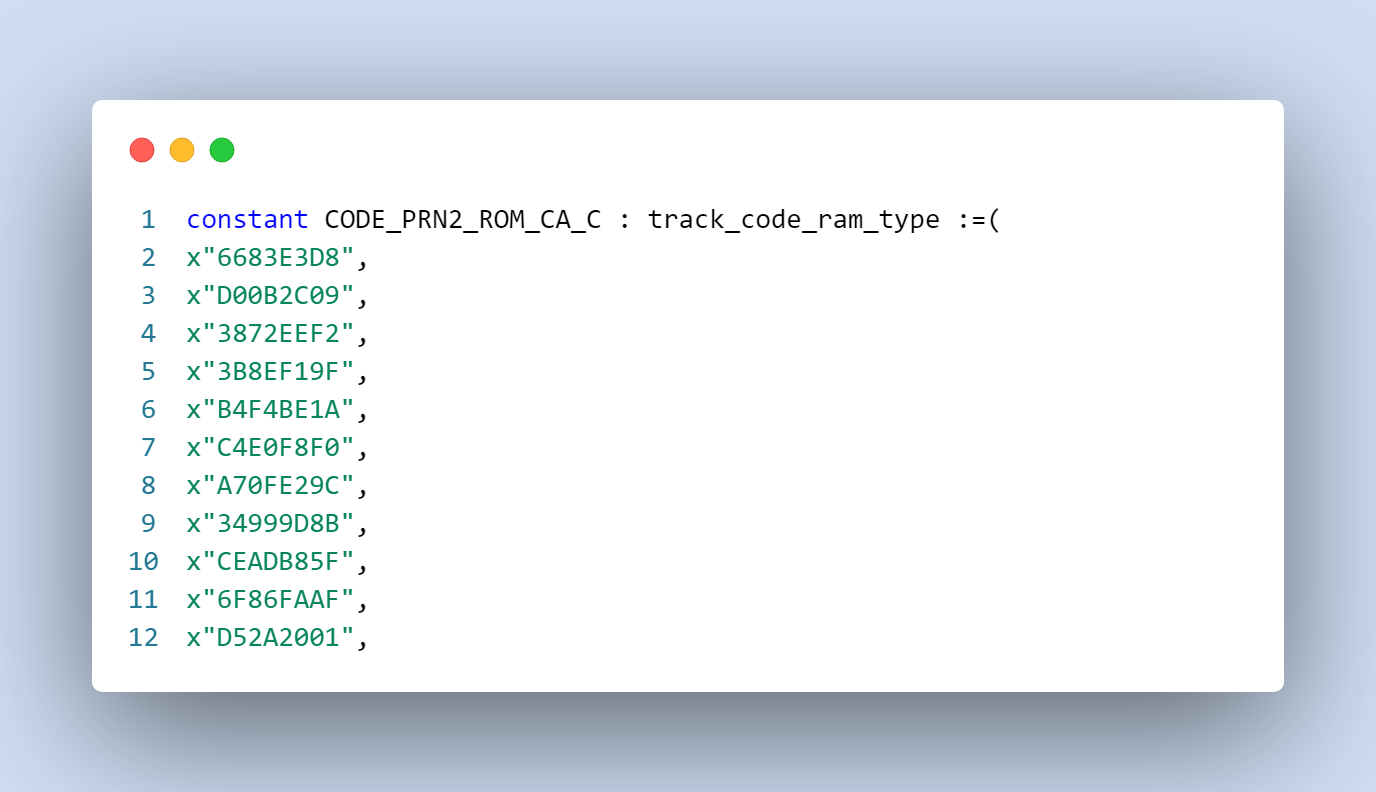
\includegraphics[width=0.5\linewidth]{_IMAGES/prn2_vhdl.png}}
    \caption{Part of the Code of PRN \textnumero 2}
    \label{fig:prn2_code}
\end{figure}

The above figures show the PRN \textnumero 2 code generated by MATLAB and the values saved in the VHDL code, which have been saved in hexadecimal, respectively.

It should also be noted that a normal PRN code should consist of 0 and 1, whereas here the 0 and 1 in the PRN code are interchanged in order to facilitate the subsequent correlator to complete the inner product calculation.

\subsection{Correlator}
The design of the correlator is at the heart of this project. The multiplier and accumulator are again at the heart of the correlator.

Our design requirement is to find the inner product of the local code and the input signal over a period of 1 ms. 
\begin{itemize}
    \item Firstly a timer of 1 ms is required, here we use a counter to determine the elapsed time by recording the number of PRN codes. When the number of PRN codes reaches 1023, then one millisecond has been reached.
    \item At the beginning of a 1 ms slot, the inner product of each bit and the current C/A code bit is stored in a register. The result of the inner product of each bit is continually accumulated until 1 ms is reached.
    \item After every 1 millisecond end, the value of the accumulation register is saved and set to zero before the next millisecond is calculated.
\end{itemize}

Note that I don't know whether the energy is mainly concentrated in phase I or phase Q, so each product operation needs to be processed separately for I/Q phase. Assuming we simulate for 60ms, we will get 60 results. Plotting these sixty results in Matlab gives results similar to figure \ref{fig:corre_function}. However, to ensure that we are tracking the correct code delay, we need three correlators that use the early, prompt, and late code to determine their results after correlation.

\subsubsection{Early, Prompt, and Late Code Generator}
\begin{figure}[!htbp]
    \centering
    \includesvg[width=0.8\textwidth]{_IMAGES/PPT2SVG/prompt_code.svg}
    \caption{Diagram of \colorbox{lightgray}{$code\_subcarr\_delay\_reg\_u$} Register}
    \label{fig:prompt_code}
\end{figure}

In order to generate the early, prompt, and late code, I design a register\\ \colorbox{lightgray}{$code\_subcarr\_delay\_reg\_u$}. It is 98 bits wide and filled with PRN \textnumero 2 code. I take the 25th bit for the early code, the 49th bit for the prompt code, and the 73rd bit for the late code. It is shown in figure \ref{fig:prompt_code}.

\subsubsection{Multiplier Optimization}
As mentioned earlier, finding the inner product is the core of the correlator, so a lot of multipliers will be used. However, compilers like Vivado will call on the on-board DSP resources to replace the multipliers during synthesis, which I don't want to see because on-board DSP resources are scarce \cite{RN208, RN209}, and they should be used elsewhere. So I can optimize the multiplier for the current project.

Since each time on the inner product is to let the current signal bit multiplied with the current C/A code bit, and the C/A code is only used in two cases are 0 and 1. When the C/A code bit is 1, the result of multiplying any number with 1 is unchanged, and when the C/A code bit is 0, I need to convert it to -1 first, and the result of multiplying any number with -1 is its opposite. In this case, rewriting the code saves a lot of on-board resources.The optimized code is shown below.
\begin{figure}[!htbp]
    \centering
    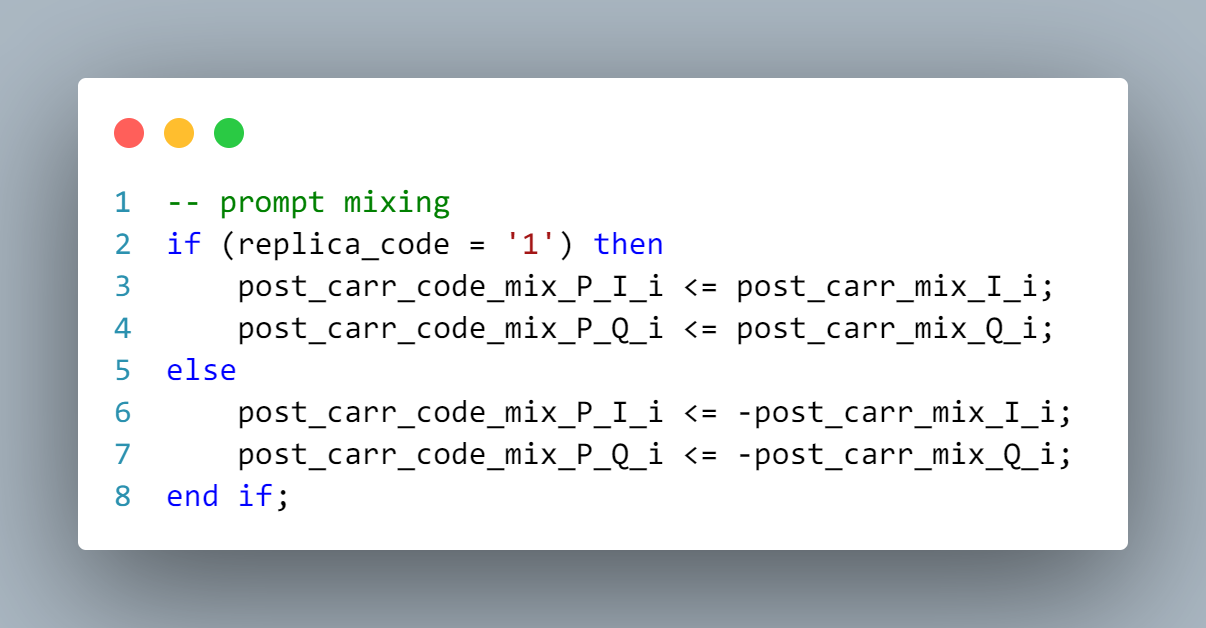
\includegraphics[width=0.9\textwidth]{_IMAGES/multiplier_code.png}
    \caption{Part of the Code of Multiplier}
    \label{fig:multiplier_code}
\end{figure}

\subsubsection{Simulation and Waveform}
Figure \ref{fig:correlator_wave} below is a waveform  of the signals mentioned above, I will explain in detail the significance of each signal and how it relates to the theory.
\begin{figure}[!htbp]
    \centering
    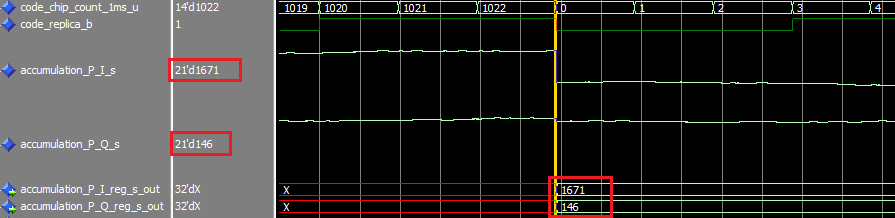
\includegraphics[width=0.9\textwidth]{_IMAGES/correlator_wave.png}
    \caption{Waveform of Key Signals in Correlator}
    \label{fig:correlator_wave}
\end{figure}

\begin{itemize}
    \item \colorbox{lightgray}{$code\_chip\_count\_1ms\_u$}: This signal is used to indicate 1 millisecond of time. It is essentially a counter that instructs the other correlation accumulation registers to store the current accumulation value by reaching a counter value of 1022, i.e. 1 milliseconds
    \item \colorbox{lightgray}{$code\_replica\_b$}:  This signal is the waveform of the PRN \textnumero 2 code output by bit.
    \item \colorbox{lightgray}{$accumulation\_P\_I\_s$}: This is the accumulation result of the I-phase prompt code, and you can see that the value has ups and downs. The result of this millisecond accumulation is \num{1671}.
    \item \colorbox{lightgray}{$accumulation\_P\_Q\_s$}: This is the accumulation result of the Q-phase prompt code, and result of this millisecond accumulation is \num{146}.
    \item \colorbox{lightgray}{$accumulation\_P\_I\_reg\_s\_out$}: This signal saves the result of this millisecond accumulation of the I-phase prompt code.
    \item \colorbox{lightgray}{$accumulation\_P\_Q\_reg\_s\_out$}: This signal saves the result of this millisecond accumulation of the Q-phase prompt code.
\end{itemize}

